
% \section{Checklist}\label{app:checklist}
% You may include other additional sections here.

\section{Our model training (\S\ref{sec:own-repl})}\label{app:our_models}

We train a variety of Transformer LMs, ranging in size from 12 million to 1 billion parameters, on FineWeb \citep{penedo2024finewebdatasetsdecantingweb}, tokenized with the GPT-NeoX-20B tokenizer \citep{black2022gptneox20bopensourceautoregressivelanguage}, which is a BPE tokenizer with a vocabulary size of 50257, trained on the Pile \citep{gao2020pile800gbdatasetdiverse}. All models were trained on a combination of NVIDIA GeForce RTX 2080 Ti, Quadro RTX 6000, NVIDIA A40, and NVIDIA L40 GPUs. These transformers follow the standard architecture, and use pre-layer RMSNorm \citep{kudo2018sentencepiece}, the SwiGLU activation function \citep{shazeer2020gluvariantsimprovetransformer}, and rotary positional embeddings \citep{su2024roformer}. We use a batch size of 512 with a sequence length of 2048. The learning rate is warmed up linearly over 50 steps to the peak learning rate and then follows a cosine decay to 10\% of the peak. We use an Adam optimizer with $\beta_1 =
0.9, \beta_2 = 0.95$. We sweep over learning rates and data budgets at each model scale. For our evaluation metric, we use perplexity on a validation set of C4 \citep{raffel2020exploring}. See Table~\ref{tab:hparams} and Table~\ref{tab:arch} for additional architecture details and hyperparameters, including data budget and learning rate.

\begin{figure*}[htbp]
    \centering%
    \setlength{\tabcolsep}{0.002\textwidth}%
    \renewcommand{\arraystretch}{1}%
    \footnotesize%
    \begin{tabular}{cccccccc}
        &Initial asset& \multicolumn{6}{c}{
            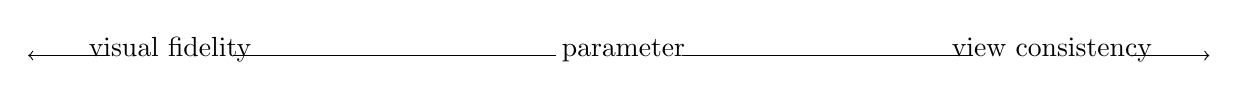
\begin{tikzpicture}
                \draw[<-] (0,0) -- (1,0);
                \draw[-] (2.6,0) -- (6.7,0);
                \draw[-] (8.3,0) -- (12,0);
                \draw[->] (14,0) -- (15,0);
                \node[above] at (1.8,-0.2) {visual fidelity};
                \node[above] at (7.5,-0.2) {$\bias$ parameter};
                \node[above] at (13,-0.2) {view consistency};
            \end{tikzpicture}
        }\\[-4pt]%
        && 0.0 & 0.6 & \textbf{1.2} & \textbf{1.8} & 2.4 & 3.0\\%
        \rotatebox{90}{\hspace*{4em}View 1}&%
        \includegraphics[height=0.14\linewidth, trim=150 0 100 0, clip]{figures/hparams_adjusting/initial_2_overlay.jpg}&%
        \includegraphics[height=0.14\linewidth, trim=200 40 300 460, clip]{figures/hparams_adjusting/0.0_2_overlay.jpg}&%
        \includegraphics[height=0.14\linewidth, trim=200 40 300 460, clip]{figures/hparams_adjusting/0.6_2_overlay.jpg}&%
        \includegraphics[height=0.14\linewidth, trim=200 40 300 460, clip]{figures/hparams_adjusting/1.2_2_overlay.jpg}&%
        \includegraphics[height=0.14\linewidth, trim=200 40 300 460, clip]{figures/hparams_adjusting/1.8_2_overlay.jpg}&%
        \includegraphics[height=0.14\linewidth, trim=200 40 300 460, clip]{figures/hparams_adjusting/2.4_2_overlay.jpg}&%
        \includegraphics[height=0.14\linewidth, trim=200 40 300 460, clip]{figures/hparams_adjusting/3.0_2_overlay.jpg}\\%
        \rotatebox{90}{\hspace*{2em}View 2, $+ 40^\circ$}&
        \includegraphics[height=0.14\linewidth, trim=150 0 100 0, clip]{figures/hparams_adjusting/initial_3_overlay.jpg}&%
        \includegraphics[height=0.14\linewidth, trim=200 40 300 460, clip]{figures/hparams_adjusting/0.0_3_overlay.jpg}&%
        \includegraphics[height=0.14\linewidth, trim=200 40 300 460, clip]{figures/hparams_adjusting/0.6_3_overlay.jpg}&%
        \includegraphics[height=0.14\linewidth, trim=200 40 300 460, clip]{figures/hparams_adjusting/1.2_3_overlay.jpg}&%
        \includegraphics[height=0.14\linewidth, trim=200 40 300 460, clip]{figures/hparams_adjusting/1.8_3_overlay.jpg}&%
        \includegraphics[height=0.14\linewidth, trim=200 40 300 460, clip]{figures/hparams_adjusting/2.4_3_overlay.jpg}&%
        \includegraphics[height=0.14\linewidth, trim=200 40 300 460, clip]{figures/hparams_adjusting/3.0_3_overlay.jpg}\\%
    \end{tabular}%
    \caption{The bias parameter $\bias$ trades between visual fidelity (left insets) and multi-view consistency (right insets). The first column shows the initial asset in two views that condition the diffusion model. The white shapes outline a UV region, which we analyze in the insets to illustrate the impact of the $\bias$ parameter on generated visuals.
    Values between 1.2 and 1.8 strike a good balance in this particular scene.}
    \label{fig:hparams}
\end{figure*}










\begin{figure}[t!]
    \newdimen\base
    \base=0.5cm
    \newdimen\xsep
    \xsep=0.3cm

    \tikzstyle{common} = [font=\scriptsize]
    \tikzstyle{split2} = [rectangle split, rectangle split parts=2, draw=black, inner sep=0pt, outer sep=0pt, minimum width=\base, minimum height=\base, inner ysep=0.5\base, rounded corners=2pt]
    
    \centering
    \begin{tikzpicture}
    
    \node[common, inner sep=0pt] (input) at (0,0) {$\nabla_{W_i}$};
    \node[common, split2, anchor=west, fill=lyyblue!40!white] (decomposein) at ([xshift=\xsep]input.east) {\rotatebox{-90}{$u_i$} \nodepart{two} \rotatebox{-90}{$\delta_{i+1}$}};
    \node[common, circle, draw=black, inner sep=1pt, anchor=west, fill=orange!30!white] (norm) at ([xshift=\xsep]decomposein.east) {norm};
    \node[common, split2, anchor=west, fill=lyyblue!40!white] (normout) at ([xshift=\xsep]norm.east) {\rotatebox{-90}{$\bar{u}_i$} \nodepart{two} \rotatebox{-90}{$\bar{\delta}_{i+1}$}};
    \node[common, trapezium, trapezium angle=30, rotate=-90, draw=black, anchor=south, fill=ugreen!30!white, minimum height=\base, minimum width=3\base, inner sep=0pt, outer sep=0pt, trapezium stretches, text width=2.5\base, align=center] (down) at ([xshift=\xsep]normout.east) {Down};
    \node[common, rectangle, draw=black, anchor=west, fill=red!30!white, minimum height=2.5\base] (hidden) at ([xshift=\xsep]down.north) {\rotatebox{-90}{Dropout}};
    \node[common, trapezium, trapezium angle=30, rotate=90, draw=black, anchor=north, fill=ugreen!30!white, minimum height=\base, minimum width=3\base, inner sep=0pt, outer sep=0pt, trapezium stretches, text width=2.5\base, align=center] (up) at ([xshift=\xsep]hidden.east) {Up};
    \node[common, anchor=west, inner sep=0pt] (residual) at ([xshift=0.7\xsep]up.south) {$\bigoplus$};
    \node[common, split2, anchor=west, fill=lyyblue!40!white] (decomposeout) at ([xshift=0.7\xsep]residual.east) {\rotatebox{-90}{$\tilde{u}_i$} \nodepart{two} \rotatebox{-90}{$\tilde{\delta}_{i+1}$}};
    \node[common, inner sep=0pt, anchor=west] (out) at ([xshift=\xsep]decomposeout.east) {$\tilde{\nabla}_{W_i}$};

    \draw[-latex] (input) to (decomposein);
    \draw[-latex] (decomposein) to (norm);
    \draw[-latex] (norm) to (normout);
    \draw[-latex] (normout) to (down);
    \draw[-latex] (down) to (hidden);
    \draw[-latex] (hidden) to (up);
    \draw[-latex] (up) to (residual);
    \draw[-latex] (residual) to (decomposeout);
    \draw[-latex] (decomposeout) to (out);

    \draw[-latex] (normout.north) |- ($(normout.north) + (0,0.5\base)$) -| (residual.north);
    
    \end{tikzpicture}
    \caption{The model architecture of \method{}.}
    \label{fig:arch}
\end{figure}

\section{Full Checklist} \label{sec:app_checklist}

% Below, we provide an expanded version of the checklist from Figure \ref{sec:checklist}. \textcolor{blue}{
We define each category as follows:
% }


\begin{itemize}
    \item {
    \textbf{Scaling Law Hypothesis:} This specifies the form of the scaling law, that of the variables and parameters, and the relation between each.}
    \item {\textbf{Training Setup:} This specifies the exact training setup of each of the models trained to test the scaling law hypothesis.}
    \item {\textbf{Data Collection:} Evaluating various checkpoints of our trained models to collect data points that will be used to fit a scaling law in the next stage.}
    \item {\textbf{Fitting Algorithm:} Using the data points collected in the previous stage to optimize the scaling law hypothesis.}
\end{itemize}


\fbox{\begin{minipage}{38em}

\subsubsection*{Scaling Law Reproducilibility Checklist}


\small

\begin{minipage}[t]{0.9\textwidth}
\raggedright
\paragraph{Scaling Law Hypothesis (\S\ref{sec:power-law-form})}

\begin{itemize}[leftmargin=*]
    \item What is the form of the power law?
    \item What are the variables related by (included in) the power law?
    \item What are the parameters to fit?
    \item On what principles is this form derived?
    \item Does this form make assumptions about how the variables are related?
    % \item How are each of these variables counted? (For example, how is compute cost/FLOPs counted, if applicable? How are parameters of the model counted?)
    % \item Are code/code snippets provided for calculating these variables if applicable? 
\end{itemize}


\paragraph{Training Setup (\S\ref{sec:model_training})}
\begin{itemize}[leftmargin=*]
    \item How many models are trained?
    \item At which sizes?
    \item On how much data each? On what data? Is any data repeated within the training for a model?
    \item How are model size, dataset size, and compute budget size counted? For example, how are parameters of the model counted? Are any parameters excluded (e.g., embedding layers)? How is compute cost calculated?
    \item Are code/code snippets provided for calculating these variables if applicable?
    \item How are hyperparameters chosen (e.g., optimizer, learning rate schedule, batch size)? Do they change with scale?
    \item What other settings must be decided (e.g., model width vs. depth)? Do they change with scale?
    \item Is the training code open source?
    % \item How is the correctness of the scaling law considered SHOULD WE?
\end{itemize}

% \end{minipage}
% \begin{minipage}[t]{0.48\textwidth}
\raggedright


\paragraph{Data Collection(\S\ref{sec:data})}
\begin{itemize}[leftmargin=*]
    \item Are the model checkpoints provided openly?
    % \item Are these checkpoints modified in any way before evaluation? (say, checkpoint averaging)
    % \item If the above is done, is code for modifying the checkpoints provided?
    \item How many checkpoints per model are evaluated to fit each scaling law? Which ones, if so?
    \item What evaluation metric is used? On what dataset?
    \item Are the raw evaluation metrics modified? Some examples include loss interpolation, centering around a mean or scaling logarithmically.
    \item If the above is done, is code for modifying the metric provided? 
\end{itemize}

\paragraph{Fitting Algorithm (\S\ref{sec:opt})}
\begin{itemize}[leftmargin=*]
    \item What objective (loss) is used?
    \item What algorithm is used to fit the equation?
    \item What hyperparameters are used for this algorithm?
    \item How is this algorithm initialized?
    \item Are all datapoints collected used to fit the equations? For example, are any outliers dropped? Are portions of the datapoints used to fit different equations?
    \item How is the correctness of the scaling law considered? Extrapolation, Confidence Intervals, Goodness of Fit?
\end{itemize}

\end{minipage}

% \paragraph{Other}
% \begin{itemize}
%     \item Is code for 
% \end{itemize}

\end{minipage}}

\pagebreak


\section{Full Sheet}\label{app:full-details}

We provide an overview of all the papers surveyed in Tables \ref{tab:full-basic},\ref{tab:full-powerlaw}, \ref{tab:full-setup}, \ref{tab:full-eval} and \ref{tab:full-opt}.


% \url{https://docs.google.com/spreadsheets/d/18RRvkRE9dNHjAnJXCIwgRk8lIwvKEfi4IK9sgscztgw/edit?gid=1894146386}



\begin{table}[!htp]
\centering
\resizebox{\textwidth}{!}{%
\begin{tabular}{lllllllll}
\toprule
Paper & Domain & Training Code? & Analysis Code? & Checkpoints? & Metric Scores? \\
\midrule
\cite{rosenfeld2019constructive} & Vision, LM & N & N & N & N \\
\cite{mikamiscaling} & Vision & N & Y & Y & Y \\
\cite{schaeffer2023emergent} & LM & N & N & N & N \\
\cite{sardana2023beyond} & LM & N & N & N & N \\
\cite{sorscher2022beyond} & Vision & N & N & N & Y \\
\cite{caballero2022broken} & LM & N & Y & N & Y \\
\cite{besiroglu2024chinchilla} & LM &  & Y & N & Y \\
\cite{gordon2021data} & NMT & Y & Y & Y & Y \\
\cite{bansal2022data} & NMT & N & N & N & N \\
\cite{hestness2017deep} & NMT, LM, Vision, Speech & N & N & N & N \\
\cite{bi2024deepseek} & LM & N & N & N & N \\
\cite{bahri2021explaining} & Vision & N & N & N & N \\
\cite{geiping2022much} & Vision & Y & Y & N & N \\
\cite{poli2024mechanistic} & LM & N & N & N & N \\
\cite{hu2024minicpm} & LM & Y & N & N & N \\
\cite{hashimoto2021model} & NLP & N & N & N & N \\
\cite{ruan2024observational} & LM & Y & Y & N & Y \\
\cite{anil2023palm} & LM & N & N & N & N \\
\cite{pearce2024reconciling} & LM & N & Y & N & N \\
\cite{cherti2023reproducible} & VLM & Y & Y & Y & Y \\
\cite{porian2024resolving} & LM & Y & Y & N & Y \\
\cite{alabdulmohsin2022revisiting} & LM, Vision & N & Y & Y & Y \\
\cite{gao2024scalingevaluatingsparseautoencoders} & NLP & Y & Y & Y & N \\
\cite{muennighoff2024scaling} & LM & Y & Y & Y & N \\
\cite{rae2021scaling} & LM & N & N & N & N \\
\cite{shin2023scaling} & RecSys & N & N & N & N \\
\cite{hernandez2022scaling} & LM & N & N & N & N \\
\cite{filipovich2022scaling} & LM & N & N & N & N \\
\cite{neumann2022scaling} & RL & Y & Y* & Y & N \\
\cite{droppo2021scaling} & Speech & N & N & N & N \\
\cite{henighan2020scaling} & LM, Vision, Video, VLM & N & N & N & N \\
\cite{goyal2024scaling} & LM, Vision, VLM & N & Y & N & Y \\
\cite{aghajanyan2023scaling} & Multimodal LM & N & N & N & N \\
\cite{kaplan2020scaling} & LM & N & N & N & N \\
\cite{ghorbani2021scaling} & NMT & N & Y & N & N \\
\cite{gao2023scaling} & RL/LM & N & N & N & N \\
\cite{hilton2023scaling} & RL & N & N & N & N \\
\cite{frantar2023scaling} & LM, Vision & N & N & N & N \\
\cite{prato2021scaling} & Vision & Y* & Y & Y & Y \\
\cite{covert2024scaling} & LM & Y & Y & N & N \\
\cite{hernandez2021scaling} & LM & N & N & N & N \\
\cite{ivgi2022scaling} & NLP & N & N & N & N \\
\cite{tay2022scaling} & LM & N & N & N & N \\
\cite{tao2024scaling} & LM & N & Y & N & Y \\
\cite{jones2021scaling} & RL & Y & Y & N & Y \\
\cite{zhai2022scaling} & Vision & Y & N & N & N \\
\cite{dettmers2023case} & LM & N & N & N & N \\
\cite{dubey2024llama} & LM & N & N & N & N \\
\cite{hoffmann2022training} & LM & N & N & N & N \\
\cite{ardalani2022understanding} & RecSys & N & N & N & N \\
\cite{clark2022unified} & LM & N & Y & N & Y \\
\bottomrule
\end{tabular}
}

\caption{Details on domain of experiments and availability of code by category for each paper surveyed.}
\label{tab:full-basic}
\end{table}

% LaTeX code for Dataframe 2:
\begin{table}[]
\centering
\resizebox{\textwidth}{!}{%
% LaTeX code for Dataframe (9, 12):
\begin{tabular}{lllll}
\toprule
Paper & Power Law Form & Purpose Of Power Law (E.G., Performance Prediction, Optimal Ratio) & \# Power Law Parameters & \# Of Scaling Laws \\
\midrule
\cite{rosenfeld2019constructive} & $\tilde{\epsilon}(m, n)=a n^{-\alpha}+b m^{-\beta}+c_{\infty}$ & Performance Prediction & 5-6 & 8 \\
\cite{mikamiscaling} & $L(n, s)=\delta\left(\gamma+n^{-\alpha}\right) s^{-\beta}$ & Performance Prediction & 4 & 3 \\
\cite{schaeffer2023emergent} & None & N/A & NA & NA \\
\cite{sardana2023beyond} & $L(N, D) = E + \frac{A}{N^\alpha} + \frac{B}{D^\beta} $; $N^*\left(\ell, D_{\text {inf }}\right), D_{\text {tr }}^*\left(\ell, D_{\text {inf }}\right)={\arg \min } _{N, D_{\mathrm{tr}} \mid L\left(N, D_{\mathrm{tr}}\right)=\ell}$ & Performance Prediction & 5 & 4 \\
\cite{sorscher2022beyond} & $c \cdot \alpha^{-\beta} ,  c \cdot \exp (-b \alpha)$ & Performance Prediction & 2 & 34 \\
\cite{caballero2022broken} & $y=a+\left(b x^{-c_0}\right) \prod_{i=1}^n\left(1+\left(\frac{x}{d_i}\right)^{1 / f_i}\right)^{-c_i * f_i}$ & Performance Prediction & 5+ & 100+ \\
\cite{besiroglu2024chinchilla} & $L(N, D) = E + \frac{A}{N^\alpha} + \frac{B}{D^\beta} $ & Performance Prediction & 5 & 1 \\
\cite{gordon2021data} & $L(N, D) = \left[ \left( \frac{N}{N_c}\right)^{\frac{\alpha_N}{\alpha_D}} + \frac{D}{D_c} \right]^{\alpha_D} $ & Performance Prediction & 4 & 3 \\
\cite{bansal2022data} & $L(D)=\alpha\left(D^{-1}+C\right)^p$ & Performance Prediction & 3 & 20 \\
\cite{hestness2017deep} & $\varepsilon(m) \sim \alpha m^{\beta_g}+\gamma$ & Performance Prediction & 3 & 17 \\
\cite{bi2024deepseek} & $\begin{aligned} M_{\mathrm{opt}} & =M_{\mathrm{base}} \cdot C^a \\ D_{\mathrm{opt}} & =D_{\mathrm{base}} \cdot C^b\end{aligned}$, $\begin{aligned} & \eta_{\mathrm{opt}}=0.3118 \cdot C^{-0.1250} \\ & B_{\mathrm{opt}}=0.2920 \cdot C^{0.3271}\end{aligned}$ & Optimal Ratio, Performance Prediction & 2 & 5 \\
\cite{bahri2021explaining} & $L(D) \propto D^{-\alpha_K}, \quad L(P) \propto P^{-\alpha_K}$ & Performance Prediction & 2 & 35 \\
\cite{geiping2022much} & $f(x)=a x^{-c}+b$, $v_{\text {Effective Extra Samples from Augmentations }}(x)=f_{\text {ref }}^{-1}\left(f_{\text {aug }}(x)\right)-x$ & Performance Prediction & 3 & ~50 \\
\cite{poli2024mechanistic} & $\log N^* \propto a \log C$ and $\log D^* \propto b \log C$ & Performance Prediction & 2 &  \\
\cite{hu2024minicpm} & $L(N, D)=C_N N^{-\alpha}+C_D D^{-\beta}+L_0$ & Performance Prediction & 5 & 6 \\
\cite{hashimoto2021model} & $\min _{\lambda, \alpha} \mathbb{E}_{\hat{q}, \hat{n}}\left[\left(\log (R(\hat{n}, \hat{q})-\epsilon)-\alpha \log (\hat{n})+\log \left(C_\lambda(\hat{q})\right)\right)^2\right]$ $R(\hat{n}, \hat{q})=\mathbb{E}\left[\ell\left(\hat{\theta}\left(p_{\hat{n}, \hat{q}}\right) ; x, y\right)\right]$ & Performance Prediction & 2+n(data mixes) & 4 \\
\cite{ruan2024observational} & $E_m \approx h \sigma\left(\beta^{\top} S_m+\alpha\right)$ & Performance Prediction & 3 &  \\
\cite{anil2023palm} & $N^{\star}(C) \approx N_0^{\star} \cdot C^a$ & Performance Prediction & 2 & 1 \\
\cite{pearce2024reconciling} & $N^*_{{\setminus E}} = b C_{{\setminus E}}^m$ $L = bC^m$ & Optimal Ratio, Performance Prediction & 2 & 1 \\
\cite{cherti2023reproducible} & $E=\beta C^{\alpha}$ & Performance Prediction & 2 & 8 \\
\cite{porian2024resolving} & $N^{\star}(C) \approx N_0^{\star} \cdot C^a$ & Optimal Ratio & 2 & 6 \\
\cite{alabdulmohsin2022revisiting} & $\varepsilon_x=\beta x^c$; $\varepsilon_x - \varepsilon_\infty=\beta x^c$; $\varepsilon_x=\beta (x^{-1} + \gamma)^{-c}$;   $\varepsilon_x=\gamma(x)(1+\gamma(x))^{-1} \varepsilon_0+(1+\gamma(x))^{-1} \varepsilon_{\infty}$ & Performance Prediction & 2-4 & ~600 \\
\cite{gao2024scalingevaluatingsparseautoencoders} & $L(n, k)=\exp \left(\alpha+\beta_k \log (k)+\beta_n \log (n)+\gamma \log (k) \log (n)\right)+\exp (\zeta+\eta \log (k))$ & Performance Prediction & 2-6 & 1 \\
\cite{muennighoff2024scaling} & $L\left(U_N, U_D, R_N, R_D\right)=\frac{A}{\left(U_N+U_N R_N^*\left(1-e^{\frac{-R_N}{R_N^*}}\right)\right)^\alpha}+\frac{B}{\left(U_D+U_D R_D^*\left(1-e^{\frac{-R_D}{R_D^*}}\right)\right)^\beta}+E$ & Performance Prediction & 2 (+4) & 1 \\
\cite{rae2021scaling} & None & Performance Prediction & N/A & N/A \\
\cite{shin2023scaling} & None & Scaling trend & NA & NA \\
\cite{hernandez2022scaling} & $E=k * N^\alpha$ & Optimal Ratio & 2 & 1 \\
\cite{filipovich2022scaling} & $\mathcal{L}(C)=\left(C_c C\right)^{\alpha_C}$ & Performance Prediction & 2 & 3 \\
\cite{neumann2022scaling} & $N_{\text {opt }}(C)=\left(\frac{C}{C_0}\right)^{\alpha_C^{o p t}}$, $E_i=\frac{1}{1+\left(N_j / N_i\right)^{\alpha_N}}$ & Performance Prediction & 2 & 3 * 2 \\
\cite{droppo2021scaling} & $L(N, D)=\left[\left(L_{\infty}\right)^{\frac{1}{\alpha}}+\left(\frac{N_C}{N}\right)^{\frac{\alpha_N}{\alpha}}+\left(\frac{D_C}{D}\right)^{\frac{\alpha_D}{\alpha}}\right]^\alpha$ & Performance Prediction & 6 & 3 \\
\cite{henighan2020scaling} & $L(x)=L_{\infty}+\left(\frac{x_0}{x}\right)^{\alpha_x}$ & Performance Prediction & 3 & 36 \\
\cite{goyal2024scaling} & $y_k=a \cdot n_1^{b_1} \prod_{j=2}^k\left(\frac{n_j}{n_{j-1}}\right)^{b_j}+d$ & Performance Prediction & 2+ 2*n(data mixes) & 1 \\
\cite{aghajanyan2023scaling} & $L(N, D_j)=E_j + \frac{A_j}{N^{\alpha_j}} + \frac{B_j}{|D_j|^{\beta_j}}$, $L(N, D_i, D_j) = [\frac{L(N, D_i) + L(N, D_j)}{2}] - C_{i,j} + \frac{A_{i,j}}{N^{\alpha_{i,j}}} + \frac{B_{i,j}}{|D_i|+|D_j|^{\beta_{i,j}}}$ & Performance Prediction & 5 & 14 \\
\cite{kaplan2020scaling} & $L(N, D) = \left[ \left( \frac{N}{N_c}\right)^{\frac{\alpha_N}{\alpha_D}} + \frac{D}{D_c} \right]^{\alpha_D}$     & Performance Prediction & 4 & ~7 \\
\cite{ghorbani2021scaling} & $\mathrm{BLEU}=c_B L^{-p_B}$, $\hat{L}_{o p t}(B)=\alpha^* B^{-\left(p_d+p_e\right)}+L_{\infty}, \quad \alpha^* \equiv \alpha\left(\frac{\bar{N}_e\left(p_e+p_d\right)}{p_e}\right)^{p_e}\left(\frac{\bar{N}_d\left(p_e+p_d\right)}{p_d}\right)^{p_d}$ & Optimal Ratio, Performance Prediction & 6 & ~8 \\
\cite{gao2023scaling} & $\begin{aligned} & R_{\mathrm{bo} n}(d)=d\left(\alpha_{\mathrm{bo} n}-\beta_{\mathrm{bo} n} d\right), \\ & R_{\mathrm{RL}}(d)=d\left(\alpha_{\mathrm{RL}}-\beta_{\mathrm{RL}} \log d\right)\end{aligned}$ & Performance Prediction & 2 & 2 \\
\cite{hilton2023scaling} & $I^{-\beta}=\left(\frac{N_c}{N}\right)^{\alpha_N}+\left(\frac{E_c}{E}\right)^{\alpha_E}$ & Optimal Ratio, Performance Prediction & 5 & 3 \\
\cite{frantar2023scaling} & $L(S, N, D)=\left(a_S(1-S)^{b_S}+c_S\right) \cdot\left(\frac{1}{N}\right)^{b_N}+\left(\frac{a_D}{D}\right)^{b_D}+c$ & Optimal Ratio, Performance Prediction & 7 & 2 \\
\cite{prato2021scaling} & $\begin{aligned} & \operatorname{Err}(N)=\operatorname{Err}_{\infty}+k N^\alpha, \\ & \operatorname{Err}(C)=\operatorname{Err}_{\infty}+k C^\alpha,\end{aligned}$ & Performance Prediction & 3 & 12 \\
\cite{covert2024scaling} & $\log \left|\psi_k(z)\right| \approx \log |c(z)|-\alpha(z) \log (k)$ & Performance Prediction & 2 & Many \\
\cite{hernandez2021scaling} & $L \approx\left[\left(\frac{N_C}{N}\right)^{\frac{\alpha_N}{\alpha_D}}+\frac{D_C}{k\left(D_F\right)^\alpha(N)^\beta}\right]^{\alpha_D}$ & Performance Prediction & 3 & 1 \\
\cite{ivgi2022scaling} & NS & Performance Prediction & NA & NA \\
\cite{tay2022scaling} & None & Scaling trend & NA & NA \\
\cite{tao2024scaling} & $N_{\mathrm{v}}^{\mathrm{opt}}=N_{\mathrm{v}}^0 *\left(\frac{N_{\mathrm{nv}}}{N_{\mathrm{nv}}^0}\right)^\gamma$, $\mathcal{L}_u=-E+\frac{A_1}{N_{\mathrm{nv}}^{\alpha_1}}+\frac{A_2}{N_{\mathrm{v}}^{\alpha_2}}+\frac{B}{D^\beta}$ & Optimal Ratio, Performance Prediction & 7 & 2 \\
\cite{jones2021scaling} & $\begin{aligned} \text { plateau } & =m_{\text {boardsize }}^{\text {plateau }} \cdot \text { boardsize }+c^{\text {plateau }} \\ \text { incline } & =m_{\text {boardsize }}^{\text {incline }} \cdot \text { boardsize }+m_{\text {flops }}^{\text {incline }} \cdot \log \text { flop }+c^{\text {incline }} \\ \text { elo } & =\text { incline.clamp }(\text { plateau }, 0)\end{aligned}$ & Performance Prediction & 5 & 1 \\
\cite{zhai2022scaling} & $E=\alpha+\beta(C+\gamma)^{-\mu}$ & Performance Prediction & 4 & 3 \\
\cite{dettmers2023case} & None & Scaling trend & NA & NA \\
\cite{dubey2024llama} & $N^{\star}(C)=A C^\alpha$. & Optimal Ratio  & 2 & 2 \\
\cite{hoffmann2022training} & A3: $L(N, D) = E + \frac{A}{N^\alpha} + \frac{B}{D^\beta} $ & Optimal Ratio, Performance Prediction & 5 & 3 \\
\cite{ardalani2022understanding} & $\left(\alpha x^{-\beta}+\gamma\right)$ & Performance Prediction & 3 & 3 \\
\cite{clark2022unified} & $\log L(N, E) \triangleq+a \log N+b \log E+c \log N \log E+d$ & Performance Prediction & 4 & 3 \\
\bottomrule
\end{tabular}
}

\caption{Details on power law for each paper surveyed.}
\label{tab:full-powerlaw}
\end{table}

% LaTeX code for Dataframe 2:
\begin{table}[]
\centering
\resizebox{\textwidth}{!}{%
% LaTeX code for Dataframe 3:
% LaTeX code for Dataframe (13, 19):
\begin{tabular}{llllllll}
\toprule
Paper & Training Runs / Law & Max. Training Flops & Max. Training Params & Max. Training Data & Data Described? & Hyperparameters Described? & How Are Model Params Counted \\
&&&&&&& (E.G., W/ Or W/Out Embeddings) \\
\midrule
\cite{rosenfeld2019constructive} & 42-49 &  & 0.7M-70M & 100M words / 1.2M images & Y & Y & Non-embedding \\
\cite{mikamiscaling} & 7 &  & ResNet-101 & 64k-1.28M images & Y & Y & NA \\
\cite{schaeffer2023emergent} & 4 &  & $10^{11}$ & NA & Y & NA & Non-embedding \\
\cite{sardana2023beyond} & 47 &  & 150M-6B & 1.5B-1.25T tokens & N & Y & NA \\
\cite{sorscher2022beyond} & ~60 &  & 86M (ViT) & 200 epochs & Y & Y & NA \\
\cite{caballero2022broken} & 3-40 &  & NS & NS & N & N & NS \\
\cite{besiroglu2024chinchilla} & NA & NA & NA & NA & Y & NA & Non-embedding \\
\cite{gordon2021data} & 45-55 &  & 56M & 28.3M-51.1M examples & Y & Y & Non-embedding \\
\cite{bansal2022data} & 10 &  & 170M-800M & 500K-512M sentences (28B tokens) & Y & Y & NS \\
\cite{hestness2017deep} & ~9 &  & upto 193M  & $2^{19}-2^{28}$ tokens, upto $2^9$ images, $2k$ audio hours & Y & Y & NS \\
\cite{bi2024deepseek} & 80 & $1e17-3e20$ &  &  & Y & Y & Non-embedding \\
\cite{bahri2021explaining} & 8-27 &  & 36.5M & upto 78k steps; 100 epochs & Y & Y & NS \\
\cite{geiping2022much} & 13 &  & ResNet-18 & upto 7.6M images & Y & Y & NS \\
\cite{poli2024mechanistic} & 500 total & 8.00E+19 & 70M-7B &  & Y & Y & Non-embedding  \\
\cite{hu2024minicpm} & 36 &  & 40M-2B & 400M-120B tokens & Y & Y & Non-embedding  \\
\cite{hashimoto2021model} &  &  &  & upto 600k sentences & Y & Y & NA \\
\cite{ruan2024observational} & 27* -77* &  & 70B-180B & 3T-6T tokens & N/A & N/A & N.S. \\
\cite{anil2023palm} & 12 & 1.00E+22 & 15B & 4.00E+11 & N & N & Non-embedding \\
\cite{pearce2024reconciling} & 20 (simulated), 25 (real) &  & 1.5B (simulated), 4.6M (real) & 23B (simulated), 500M (real) tokens & Y & Y & w/ Embedding and Non-embedding considered separately \\
\cite{cherti2023reproducible} & 3* - 29 &  & 214M & 34B (pretrain), 2B (finetune) examples  & Y & Y & N.S \\
\cite{porian2024resolving} & 16 & 2.00E+19 & 901M &  & Y & Y & w/ Embedding and Non-embedding considered separately \\
\cite{alabdulmohsin2022revisiting} & 1* &  & 110M-1B & 1e6-1e10 ex / 3e11 tokens & Mixed & N & N/A \\
\cite{gao2024scalingevaluatingsparseautoencoders} & N.S & N.S & N.S & N.S & N & N & N.S \\
\cite{muennighoff2024scaling} & 142 &  & 8,7B & 900B tokens & Y & Y & w/ embedding \\
\cite{rae2021scaling} & 4 & 6.31E+23 & 280B &  & Y & Y & Non-embedding \\
\cite{shin2023scaling} & 17 & ~0.1 PF Days & 160M & 500M-50B tokens & Y & Y & NA \\
\cite{hernandez2022scaling} & 56 &  & 1.5M-800M & 100B tokens & N & N & NS \\
\cite{filipovich2022scaling} & 4 &  & 57-509M & 30B token & Y & N & NS \\
\cite{neumann2022scaling} & 14 &  & ~$5*10^5$ & $10^4$ steps & Y & Y & NS \\
\cite{droppo2021scaling} & 5-21 &  & ~$10^7$ & 134-23k hrs speech & Y & Y & NS \\
\cite{henighan2020scaling} & 6-10 &  & ~$10^11$ & ~$10^12$ tokens & Y & Y & Non-embedding \\
\cite{goyal2024scaling} & 5 &  & CLIP L/14 - ~300M +63M & 32-640M samples & Y & Y & Embedding \\
\cite{aghajanyan2023scaling} & 21 &  & 8M-6.7B & 5-100B tokens & Y & Y & Non-embedding \\
\cite{kaplan2020scaling} & ~40-150 &  & 1.5B & 23B tokens & Y & Y & Non-embedding \\
\cite{ghorbani2021scaling} & 12-14 &  & 191-3B & NS & Y & Y & Non-embedding \\
\cite{gao2023scaling} & 9 &  & 3B & 120-90k & N & Y & NS \\
\cite{hilton2023scaling} & NS & $10^{20}$ &  &  & Y & Y & NS \\
\cite{frantar2023scaling} & 48 and 112 &  & 0.66M-85M  & 1.8B images, 65B tokens & Y & Y & Non-embedding \\
\cite{prato2021scaling} & 5 &  &  & $10^6$ samples & Y & N & NA \\
\cite{covert2024scaling} & 10 &  & NA & 1000 samples for IMDB & Y & Y & NA \\
\cite{hernandez2021scaling} & NS & $10^{21}$ & $10^8$ &  & Y & N & Non-embedding \\
\cite{ivgi2022scaling} & 5-8 &  & $10^4-10^8$ & varies; 500k steps PT & Y & Y & Non-embedding \\
\cite{tay2022scaling} &  &  & 16-30B & $2^19$ & Y & Y & NA \\
\cite{tao2024scaling} & 60 &  & 33M-1.13B NV + 4-96k V & 4.3B-509B Characters & Y & Y & Embedding and Non-embedding considered separately \\
\cite{jones2021scaling} & 200 & 1E+12-1E+17 &  & 4E+08-2E+09 & Y & Y & NA \\
\cite{zhai2022scaling} & 44 &  & 5.4M-1.8B & 1-13M images & Y & Y & NA \\
\cite{dettmers2023case} & 4 &  & 19M-176B & NA & NA & Y & NA \\
\cite{dubey2024llama} & NS & $6*10^{18}-10^22$ & 40M-16B &  & Y* & Y & NS \\
\cite{hoffmann2022training} & ~200-450 & $6*10^{18}-3*10^{21}$ & 16B & 5B-400B tokens & Y & Y & Non-embedding \\
\cite{ardalani2022understanding} & NS & $10^2$-$10^6$ TFlops &  & ~5M-5B samples & N & N & All are considered \\
\cite{clark2022unified} & 56 &  & 15M-1.3B & 130B tokens & Y & Y & Non-embedding \\
\bottomrule
\end{tabular}

}

\caption{Details on training setup for each paper surveyed.}
\label{tab:full-setup}
\end{table}

% LaTeX code for Dataframe 2:
\begin{table}[]
\centering
\resizebox{\textwidth}{!}{%

% LaTeX code for Dataframe (20, 24):
\begin{tabular}{lllll}
\toprule
Paper & Data Points Per Law? & Scaling Law Metric & Modification Of Final Metric? & Subsets Of Data Used \\
\midrule
\cite{rosenfeld2019constructive} & 42-49 & Loss / Top1 Error & N & N \\
\cite{mikamiscaling} & 7 & Error Rate & N & N \\
\cite{schaeffer2023emergent} & NA & Various downstream & NA & NA \\
\cite{sardana2023beyond} & NS & Loss & NS & NS \\
\cite{sorscher2022beyond} & ~60 & Error Rate & NA & NA \\
\cite{caballero2022broken} & 3-40 & FID, Loss, Error Rate, Elo Score & N & NS \\
\cite{besiroglu2024chinchilla} & 245 & Loss & N & N \\
\cite{gordon2021data} & 45-55 & Loss & N & N \\
\cite{bansal2022data} & NS & Loss, BLEU & NS & NS \\
\cite{hestness2017deep} & NS & Token Error, CER, Error Rate, Loss & Median min. validation error across multiple training runs with separate random seeds & NS \\
\cite{bi2024deepseek} & upto 80 & Validation bits-per-byte & NS & NS \\
\cite{bahri2021explaining} & upto 100 & Loss & NS & NS \\
\cite{geiping2022much} & ~50 & Effective Extra Samples & Interpolation & NS \\
\cite{poli2024mechanistic} & NS & Loss & NS & NS \\
\cite{hu2024minicpm} & NS & Loss & NS & NS \\
\cite{hashimoto2021model} & NS & Loss & NS & NS \\
\cite{ruan2024observational} &  & Various downstream & N & N \\
\cite{anil2023palm} & 12 & Loss & N & N \\
\cite{pearce2024reconciling} & 20, 5 & Loss & N & N \\
\cite{cherti2023reproducible} & 3-29 & Error Rate & N & N \\
\cite{porian2024resolving} & 12 & Loss & N & N \\
\cite{alabdulmohsin2022revisiting} & N.S. & Loss / Accuracy & N & N/A \\
\cite{gao2024scalingevaluatingsparseautoencoders} & N.S & MSE & N.S & N.S \\
\cite{muennighoff2024scaling} & 142 & Loss & N & Outliers removed \\
\cite{rae2021scaling} & 4 & Loss & N/A & N/A \\
\cite{shin2023scaling} & NA & Loss & NA & NA \\
\cite{hernandez2022scaling} & NS & Loss & N & N \\
\cite{filipovich2022scaling} & NS & Loss & N & N \\
\cite{neumann2022scaling} & 238 & Elo Score & N & N \\
\cite{droppo2021scaling} & NS & Loss & N & N \\
\cite{henighan2020scaling} & NS & Loss, Error Rate & NS & Drop smaller models \\
\cite{goyal2024scaling} & NS & Error Rate & N & N \\
\cite{aghajanyan2023scaling} & NS & Perplexity & N & N \\
\cite{kaplan2020scaling} & NS & Loss & NS & NS \\
\cite{ghorbani2021scaling} & NS & Loss, BLEU & Median of last 50k steps &  \\
\cite{gao2023scaling} & ~90 & RM Score & NS & NS \\
\cite{hilton2023scaling} & NS & Intrinsic Performance & Smoothing learning curve & Exclude early checkpoints \\
\cite{frantar2023scaling} & 48 and 112 & Loss & NS & NS \\
\cite{prato2021scaling} & 5 & Error Rate & NS & NS \\
\cite{covert2024scaling} & (1000-5000 )*10 & Expectation  & NS & N \\
\cite{hernandez2021scaling} & 40-120 & Loss & NS & NS \\
\cite{ivgi2022scaling} & 5-8 & Loss & N & [2.5, 97.5] percentile \\
\cite{tay2022scaling} & NA & Loss, Accuracy & NA & NA \\
\cite{tao2024scaling} & 20*60 & Loss & Interpolation & NS \\
\cite{jones2021scaling} & 2800 & Elo Score & NS & NS \\
\cite{zhai2022scaling} & NS & Accuracy & NS & NS \\
\cite{dettmers2023case} & NA & Accuracy & NA & NA \\
\cite{dubey2024llama} & ~150 & Loss, Accuracy & NS & NS \\
\cite{hoffmann2022training} & upto 1500 & Loss & N & Lowest loss model of a FLOP count, last 15\% of checkpoints \\
\cite{ardalani2022understanding} & ~130 & Loss & NS & NS \\
\cite{clark2022unified} & ~26*56 & Loss & Log & NS \\
\bottomrule
\end{tabular}

}

\caption{Details on data extraction for each paper surveyed.}
\label{tab:full-eval}
\end{table}




\begin{table}[]
\centering
\resizebox{\textwidth}{!}{%
% LaTeX code for Dataframe (25, 29):
\begin{tabular}{llllll}
\toprule
Paper & Curve-Fitting Method & Loss Objective & Hyperparameters Reported? & Initialization & Are Scaling Laws Validated? \\
\midrule
\cite{rosenfeld2019constructive} & Least Squares Regression & Custom error term & N/A & Random & Y \\
\cite{mikamiscaling} & Non-linear Least Squares in log-log space &  & N/A & N/A & Y \\
\cite{schaeffer2023emergent} & NA & NA & NA & NA & NA \\
\cite{sardana2023beyond} & L-BFGS & Huber Loss & Y & Grid Search & N \\
\cite{sorscher2022beyond} & NA & NA & NA & NA & NA \\
\cite{caballero2022broken} & Least Squares Regression & MSLE & N/A & Grid Search, optimize one & Y \\
\cite{besiroglu2024chinchilla} & L-BFGS & Huber Loss & Y & Grid Search & Y \\
\cite{gordon2021data} & Least Squares Regression &  & N/A & N.S. & N \\
\cite{bansal2022data} & NS & NS & N & NS & N \\
\cite{hestness2017deep} & NS & RMSE & N & NS & Y \\
\cite{bi2024deepseek} & NS & NS & N & NS & Y \\
\cite{bahri2021explaining} & NS & NS & N & NS & N \\
\cite{geiping2022much} & Non-linear Least Squares &  & NA & Non-augmented parameters & Y \\
\cite{poli2024mechanistic} & NS & NS & N & NS & N \\
\cite{hu2024minicpm} & scipy curvefit & NS & N & NS & N \\
\cite{hashimoto2021model} & Adagrad & Custom Loss & Y & Xavier & Y \\
\cite{ruan2024observational} & Linear Least Squares & Various & N/A & N/A & Y \\
\cite{anil2023palm} & Polynomial Regression (Quadratic) & N.S. & N & N.S. & Y \\
\cite{pearce2024reconciling} & Polynomial Least Squares & MSE on Log-loss & N/A & N/A & N \\
\cite{cherti2023reproducible} & Linear Least Squares & MSE & N/A & N/A & N \\
\cite{porian2024resolving} & Weighted Linear Regression & weighted SE on Log-loss & N/A & N/A & Y \\
\cite{alabdulmohsin2022revisiting} & Least Squares Regression & MSE & Y & N.S. & Y \\
\cite{gao2024scalingevaluatingsparseautoencoders} & N.S & N.S & N.S & N.S & N.S \\
\cite{muennighoff2024scaling} & L-BFGS & Huber on Log-loss & Y & Grid Search, optimize all & Y \\
\cite{rae2021scaling} & None & None & N/A & N/A & N \\
\cite{shin2023scaling} & NA & NA & NA & NA & NA \\
\cite{hernandez2022scaling} & NS & NS & NS & NS & NS \\
\cite{filipovich2022scaling} & NS & NS & NS & NS & NS \\
\cite{neumann2022scaling} & NS & NS & NS & NS & NS \\
\cite{droppo2021scaling} & NS & NS & NS & NS & NS \\
\cite{henighan2020scaling} & NS & NS & NS & NS & NS \\
\cite{goyal2024scaling} & Grid Search & L2 error & Y & NA & Y \\
\cite{aghajanyan2023scaling} & L-BFGS & Huber on Log-loss & Y & Grid Search, optimize all & Y \\
\cite{kaplan2020scaling} & NS & NS & NS & NS & N \\
\cite{ghorbani2021scaling} & Trust Region Reflective algorithm, Least Squares & Soft-L1 Loss & Y & Fixed & Y \\
\cite{gao2023scaling} & NS & NS & NS & NS & Y \\
\cite{hilton2023scaling} & CMA-ES+Linear Regression & L2 log loss & Y & Fixed & Y \\
\cite{frantar2023scaling} & BFGS & Huber on Log-loss & Y & N Random Trials & Y \\
\cite{prato2021scaling} & NS & NS & NS & NS & NS \\
\cite{covert2024scaling} & Adam & Custom Loss & Y & NS & Y \\
\cite{hernandez2021scaling} & NS & NS & NS & NS & Y \\
\cite{ivgi2022scaling} & Linear Least Squares in Log-Log space & MSE & NA & NS & Y \\
\cite{tay2022scaling} & NA & NA & NA & NA & NA \\
\cite{tao2024scaling} & L-BFGS, Least Squares & Huber on Log-loss & Y & N Random Trials from Grid & Y \\
\cite{jones2021scaling} & L-BFGS & NS & NS & NS & NS \\
\cite{zhai2022scaling} & NS & NS & NS & NS & NS \\
\cite{dettmers2023case} & NA & NA & NA & NA & NA \\
\cite{dubey2024llama} & NS & NS & NS & NS & Y \\
\cite{hoffmann2022training} & L-BFGS & Huber on Log-loss & Y & Grid Search, optimize all & Y \\
\cite{ardalani2022understanding} & NS & NS & NS & NS & NS \\
\cite{clark2022unified} & L-BFGS-B & L2 Loss & Y & Fixed & NS \\
\bottomrule
\end{tabular}

}

\caption{Details on optimization for each paper surveyed.}
\label{tab:full-opt}
\end{table}

\newpage

\section{Recommendations}\label{sec:app_recs}

% \textcolor{blue}{
As seen in our analyses, many decisions in our checklist have a number of reasonable options, but those reasonable choices lead to a wide range of scaling law fits, and the observed variations do not follow any clear pattern. It is probable that variations would be even harder to predict when varying model architectures or other design decisions, removing the possibility of a universal set of best practices.
However, it is certainly possible to determine that some scaling law fits are plausible or highly implausible, and to observe the stability of the fitting procedure. 
% For example, in Figure 2(a), neither of the recommended data/parameters ratios of ~1/2200 or 3000/1 at $10^25$ FLOPs are likely to be the true optimal settings, and the loss predictions at those points are also unlikely to be close to ground truth. 
With the caveat that following any recommendations can not guarantee good scaling law fit, we can make some more concrete recommendations based on these observations:
\paragraph{Scaling Law Hypothesis}
\begin{itemize}
    \item Fitting fewer scaling law parameters at a time typically results in greater stability. In some cases, it may be beneficial to decompose the scaling law fitting problem into two separate procedures. Examples of this approach are the IsoFLOP procedure from \citet{hoffmann2022training}, as well as fitting first the relation between $L$ and $C$, then finding the optimal $N$ and $D$ for a $C$, as seen in \citet{porian2024resolving}.
    % \item lr
\end{itemize}
\paragraph{Training Setup}
\begin{itemize}
    \item The trained models should include a wide range of input variables settings. For example, when the input variables to the scaling law are $L$, $N$, $D$, the included models should include a wide range of $N$ and $D$ values for each $C$, or equivalently, should include a wide range of $D/N$ ratios. If the included settings do not include the true optimum, the procedure will struggle to fit to the optimum.
    \item Sweeping for the optimal learning rate results in a less stable fit than fixing the learning rate. We hypothesize that this may be because the true optimal learning rate for each model and data budget size is not any of the options we consider, and thus, each model varies in the difference between its true and approximate optimal learning rate. This may introduce additional noise to the data. Due to resource constraints, we are unable to fully test this hypothesis, and it may not hold at significantly larger scale, but we recommend fixing the learning rate, or changing it according to, say, model size, according to a fixed formula.
\end{itemize}
\paragraph{Data Collection}
\begin{itemize}
    \item Results across tasks or datasets should not be mixed. Neither performance predictions nor optimal $D/N$ ratios are fixed across different evaluation settings for the same set of models.
\end{itemize}
\paragraph{Fitting Algorithm}
\begin{itemize}
    \item Scaling law fitting is sensitive to initialization; most known optimization methods for scaling laws are only able, in practice, to the shift parameters near to their initialization values. Thus, a  dense search over initialization values is necessary. If there is a strong hypothesis guiding the choice of one specific initialization, such as a previously fit and validated scaling law, this will also limit the set of possible final scaling law parameter values.
    \item Different losses emphasize the contribution of errors from certain datapoints. The chosen loss should be suited to the distribution of datapoints and sources of noise.
    \item A simple grid search is unlikely to result in a good scaling law fit. Additionally, optimizers designed to fit linear relations may make assumptions about the distribution of errors and should not be used to fit a power law. 
\end{itemize}
% }


\subsection{Example Checklist}

% \vspace{-5cm}
% \textcolor{blue}{
We provide one possible set of responses to our checklist, reflective of some recommendations enumerated above, and loosely based on \citet{hoffmann2022training}. These answers roughly correspond to a subset of the experiments we run in \S\ref{sec:own-repl}.
% }

\newpage

\fbox{\begin{minipage}[!ht]{38em}

\subsubsection*{(Mis)Fitting: Scaling Law Reproducibility Checklist}


\small

\begin{minipage}[!htp]{0.95\textwidth}
\raggedright
\paragraph{Scaling Law Hypothesis (\S\ref{sec:power-law-form})}

\begin{itemize}[leftmargin=*]
    \item What is the form of the power law? \textit{$L(N, D) = E + \frac{A}{N^\alpha} + \frac{B}{D^\beta} $}
    \item What are the variables related by (included in) the power law? \textit{$N$: the number of model parameters, $D$: the number of data tokens, and $L$: the model's validation loss}
    \item What are the parameters to fit? \textit{$A$, $B$, $E$, $\alpha$, $\beta$}
    \item On what principles is this form derived? \textit{This is taken from \citet{hoffmann2022training}, who hypothesize this form on the basis of prior work in risk decomposition.}
    \item Does this form make assumptions about how the variables are related? \textit{This form inherently assumes that $N$ and $D$ do not have any interaction in their effect on the scaling of $L$. For some experiments, we use the assumption $\alpha = \beta$ to simplify optimization.}
    % \item How are each of these variables counted? (For example, how is compute cost/FLOPs counted, if applicable? How are parameters of the model counted?)
    % \item Are code/code snippets provided for calculating these variables if applicable? 
\end{itemize}


\paragraph{Training Setup (\S\ref{sec:model_training})}
\begin{itemize}[leftmargin=*]
    \item How many models are trained?
    \textit{Refer to Table 10}
    \item At which sizes?
    \textit{Refer to Table 10}
    \item On how much data each? On what data? Is any data repeated within the training for a model?
    \textit{Refer to Table 10.}
    \item How are model size, dataset size, and compute budget size counted? For example, how are parameters of the model counted? Are any parameters excluded (e.g., embedding layers)? How is compute cost calculated?  \textit{We include the results including and excluding embedding layers for both the total parameter count $N$ and the total FLOP count $C$. We also include, for comparison, results using the estimate $C=6ND$.}
    \item Are code/code snippets provided for calculating these variables if applicable?
    \url{https://github.com/hadasah/scaling_laws}
    \item How are hyperparameters chosen (e.g., optimizer, learning rate schedule, batch size)? Do they change with scale? \textit{Most hyperparameters are chosen based on best practices in current literature; several are taken directly from the settings in \citet{hoffmann2022training}. For learning rate, we conduct an extensive hyperparameter search across 2-3 orders of magnitude, multiplying by 2-2.5, and then conduct training at 3 learning rates, including the optimum, for nearly all ($N$, $D$) configurations.}
    \item What other settings must be decided (e.g., model width vs. depth)? Do they change with scale?  
    \textit{Refer to Table 10}
    \item Is the training code open source?
    \textit{Yes}
\end{itemize}

\begin{figure}[t!]
    \newdimen\base
    \base=0.5cm
    \newdimen\xsep
    \xsep=0.3cm

    \tikzstyle{common} = [font=\scriptsize]
    \tikzstyle{split2} = [rectangle split, rectangle split parts=2, draw=black, inner sep=0pt, outer sep=0pt, minimum width=\base, minimum height=\base, inner ysep=0.5\base, rounded corners=2pt]
    
    \centering
    \begin{tikzpicture}
    
    \node[common, inner sep=0pt] (input) at (0,0) {$\nabla_{W_i}$};
    \node[common, split2, anchor=west, fill=lyyblue!40!white] (decomposein) at ([xshift=\xsep]input.east) {\rotatebox{-90}{$u_i$} \nodepart{two} \rotatebox{-90}{$\delta_{i+1}$}};
    \node[common, circle, draw=black, inner sep=1pt, anchor=west, fill=orange!30!white] (norm) at ([xshift=\xsep]decomposein.east) {norm};
    \node[common, split2, anchor=west, fill=lyyblue!40!white] (normout) at ([xshift=\xsep]norm.east) {\rotatebox{-90}{$\bar{u}_i$} \nodepart{two} \rotatebox{-90}{$\bar{\delta}_{i+1}$}};
    \node[common, trapezium, trapezium angle=30, rotate=-90, draw=black, anchor=south, fill=ugreen!30!white, minimum height=\base, minimum width=3\base, inner sep=0pt, outer sep=0pt, trapezium stretches, text width=2.5\base, align=center] (down) at ([xshift=\xsep]normout.east) {Down};
    \node[common, rectangle, draw=black, anchor=west, fill=red!30!white, minimum height=2.5\base] (hidden) at ([xshift=\xsep]down.north) {\rotatebox{-90}{Dropout}};
    \node[common, trapezium, trapezium angle=30, rotate=90, draw=black, anchor=north, fill=ugreen!30!white, minimum height=\base, minimum width=3\base, inner sep=0pt, outer sep=0pt, trapezium stretches, text width=2.5\base, align=center] (up) at ([xshift=\xsep]hidden.east) {Up};
    \node[common, anchor=west, inner sep=0pt] (residual) at ([xshift=0.7\xsep]up.south) {$\bigoplus$};
    \node[common, split2, anchor=west, fill=lyyblue!40!white] (decomposeout) at ([xshift=0.7\xsep]residual.east) {\rotatebox{-90}{$\tilde{u}_i$} \nodepart{two} \rotatebox{-90}{$\tilde{\delta}_{i+1}$}};
    \node[common, inner sep=0pt, anchor=west] (out) at ([xshift=\xsep]decomposeout.east) {$\tilde{\nabla}_{W_i}$};

    \draw[-latex] (input) to (decomposein);
    \draw[-latex] (decomposein) to (norm);
    \draw[-latex] (norm) to (normout);
    \draw[-latex] (normout) to (down);
    \draw[-latex] (down) to (hidden);
    \draw[-latex] (hidden) to (up);
    \draw[-latex] (up) to (residual);
    \draw[-latex] (residual) to (decomposeout);
    \draw[-latex] (decomposeout) to (out);

    \draw[-latex] (normout.north) |- ($(normout.north) + (0,0.5\base)$) -| (residual.north);
    
    \end{tikzpicture}
    \caption{The model architecture of \method{}.}
    \label{fig:arch}
\end{figure}

\raggedright

\end{minipage}

\end{minipage}}

\fbox{\begin{minipage}[!ht]{38em}

\small

\begin{minipage}[!ht]{0.9\textwidth}
\raggedright

\paragraph{Data Collection(\S\ref{sec:data})}
\begin{itemize}[leftmargin=*]
    \item Are the model checkpoints provided openly?
    % \item Are these checkpoints modified in any way before evaluation? (say, checkpoint averaging)
    % \item If the above is done, is code for modifying the checkpoints provided?
    \textit{Yes, at  \url{https://github.com/hadasah/scaling_laws}}
    \item How many checkpoints per model are evaluated to fit each scaling law? Which ones, if so?  \textit{Unless clearly denoted otherwise, one checkpoint per model is evaluated; the last checkpoint. By default, no mid-training checkpoints are used, i.e., from before the termination of the cosine learning rate schedules.}
    \item What evaluation metric is used? On what dataset?  \textit{We use cross-entropy loss, measured on a held-out validation subset of the Common Crawl \citep{raffel2020exploring} dataset.}
    \item Are the raw evaluation metrics modified? Some examples include loss interpolation, centering around a mean or scaling logarithmically.  \textit{No.}
    \item If the above is done, is code for modifying the metric provided? 
    \textit{Yes.}
\end{itemize}


\paragraph{Fitting Algorithm (\S\ref{sec:opt})}
\begin{itemize}[leftmargin=*]
    \item What objective (loss) is used? \textit{We try various loss objectives (1) log-Huber loss, (2) MSE, (3) MAE and (4) Huber loss}
    \item What algorithm is used to fit the equation? \textit{Mainly L-BFGS, but we also experiment with BFGS, non-linear least squares and grid search.}
    \item What hyperparameters are used for this algorithm? \textit{Thresholds of $\{1e-4, 1e-6, 1e-8\}$, exact gradient }
    \item How is this algorithm initialized? \textit{We initialize with 4500 initializations similar to \citet{hoffmann2022training}.}
    \item Are all datapoints collected used to fit the equations? For example, are any outliers dropped? Are portions of the datapoints used to fit different equations? \textit{No outliers are dropped in general, but we do show some results on specific subsets of models. For example, we compare the result of a scaling law fit when using only models trained at a peak learning rate of $1e-4$ or $4e-4$.}
    \item How is the correctness of the scaling law considered? Extrapolation, Confidence Intervals, Goodness of Fit? \textit{Currently, we do not evaluate the correctness beyond comparing to results in literature \citep{hoffmann2022training,kaplan2020scaling}.}
\end{itemize}

\end{minipage}

% \paragraph{Other}
% \begin{itemize}
%     \item Is code for 
% \end{itemize}

\end{minipage}}

\newpage


\section{Full Analysis Plots}\label{sec:app_megafigure}

\begin{figure}[!htp]
\centering
\begin{subfigure}{\textwidth}
    \centering
\begin{subfigure}{0.49\textwidth}
    \includegraphics[width=\textwidth]{images/analysis_form_epoch_ai_C_vs_N.pdf}  \footnotesize{\citet{hoffmann2022training,besiroglu2024chinchilla}}
\end{subfigure}
\\ \vspace{1em}
\centering
\begin{subfigure}{0.49\textwidth}
    \centering
    \includegraphics[width=\textwidth]{images/analysis_form_rsld_final_C_vs_N.pdf}
    \footnotesize{\citet{porian2024resolving}}
\end{subfigure}
\hfill
\begin{subfigure}{0.49\textwidth}
    \centering
    \includegraphics[width=\textwidth]{images/analysis_form_rsld_ckpt_C_vs_N.pdf}
    \footnotesize{\citet{porian2024resolving} (all checkpoints)}
\end{subfigure}
\\ \vspace{1em}
\centering
\begin{subfigure}{0.49\textwidth}
    \centering
    \includegraphics[width=\textwidth]{images/analysis_form_misfitting_new_final_C_vs_N.pdf}
    \footnotesize{Ours}
\end{subfigure}
    \hfill
\begin{subfigure}{0.49\textwidth}
    \centering
    \includegraphics[width=\textwidth]{images/analysis_form_misfitting_new_ckpt_C_vs_N.pdf}
    \footnotesize{Ours (all checkpoints)}
\end{subfigure}
\\ \vspace{1em}
\caption{\textbf{\S\ref{sec:power-law-form}, \S\ref{sec:repl-power-law-form}} Using data from both \citet{besiroglu2024chinchilla} (left) and our own models (right), we compare the effects of fitting to the power law form used in Approach 3 of \citet{hoffmann2022training} with the variant used by \citet{muennighoff2024scaling}, which assumes that the exponents $\alpha, \beta$ are equal -- equivalently, that $N^*(C)$ and $D^*(C)$ scale about linearly with each other.  When using only the performance of final checkpoints from both \citet{besiroglu2024chinchilla} and our own experiments, taking this assertion results in a law much closer to the one reported by \citet{hoffmann2022training}. On our own models, we also show results when using the IsoFLOP approach from \citet{hoffmann2022training}. As we are using only results from final model checkpoints, the size of the data input to the IsoFLOP approach in this case is reduced.}
\label{fig:analysis_form_app}
\end{subfigure}
\end{figure}

\begin{figure}[]
\ContinuedFloat 
    \centering
\begin{subfigure}{\textwidth}
\begin{subfigure}{0.49\textwidth}
    \centering
    \includegraphics[width=\textwidth]{images/analysis_lr_misfitting_new_final_C_vs_N.pdf}
    \footnotesize{Ours}
\end{subfigure}
    \hfill
\begin{subfigure}{0.49\textwidth}
    \centering
    \includegraphics[width=\textwidth]{images/analysis_lr_misfitting_new_ckpt_C_vs_N.pdf}
    \footnotesize{Ours (all checkpoints)}
\end{subfigure}
    \caption{\textbf{\S\ref{sec:model_training}, \S\ref{sec:repl-model_training}} With our models, we simulate the effects of not sweeping the learning rate. As a baseline, (1) we sweep at each ($N$, $D$) pair for the optimal learning rate over a range of values at most a multiple of 2 apart. Next, (2) we use a learning rate of 1e-3 for all $N$, the optimal for our 1 billion parameter models, and do the same for (3) 2e-3 and (4) 4e-3, which is optimal for our 12 million parameter models. Lastly, we use all models across all learning rates at the same $N$ and $D$. Results vary dramatically across these settings. Somewhat surprisingly, using all learning rates results in a very similar power law to sweeping the learning rate, whereas using a fixed learning rate of 1e-3 or 4e-3 yields the lowest optimization loss or closest match to the \citet{hoffmann2022training} power laws, respectively.}
\end{subfigure}
\end{figure}

\begin{figure}[]
\ContinuedFloat
\centering 
\begin{subfigure}{\textwidth}
    \centering
\begin{subfigure}{0.49\textwidth}
    \centering
    \includegraphics[width=\textwidth]{images/analysis_dn_ratio_epoch_ai_C_vs_N.pdf}
\footnotesize{\citet{hoffmann2022training,besiroglu2024chinchilla}}
\end{subfigure}
\\ \vspace{1em}
\begin{subfigure}{0.49\textwidth}
    \centering
    \includegraphics[width=\textwidth]{images/analysis_dn_ratio_rsld_final_C_vs_N.pdf}
    \footnotesize{\citet{porian2024resolving}}
\end{subfigure}
\hfill
\begin{subfigure}{0.49\textwidth}
    \centering
    \includegraphics[width=\textwidth]{images/analysis_dn_ratio_rsld_ckpt_C_vs_N.pdf}
    \footnotesize{\citet{porian2024resolving} (all checkpoints)}
\end{subfigure}
\\ \vspace{1em}
    \centering
\begin{subfigure}{0.49\textwidth}
    \centering
    \includegraphics[width=\textwidth]{images/analysis_dn_ratio_misfitting_new_final_C_vs_N.pdf}
    \footnotesize{Ours}
\end{subfigure}
\hfill 
\begin{subfigure}{0.49\textwidth}
    \centering
    \includegraphics[width=\textwidth]{images/analysis_dn_ratio_misfitting_new_ckpt_C_vs_N.pdf}
    \footnotesize{Ours (all checkpoints)}
\end{subfigure}
\\ \vspace{1em}
\caption{\textbf{\S\ref{sec:model_training}, \S\ref{sec:repl-model_training}} From all 3 datasets, we choose subsets with ($N$, $D$) values which fit a particular method one might have of setting up training. We fit with (1) all models, which for our dataset, ranges from 12 million to 1 billion parameters, then with (2) only models of up to about 100 million parameters or (3) up to 400 million parameters. We also compare the effects of a higher or lower hypothesis about the optimal $D/N$ ratio, including (4) only models with $D/N \leq 18$ or (5) $D/N \geq 22$. These ranges are designed to exclude $D/N = 20$, the rule of thumb based on \citet{hoffmann2022training}. The minimum or maximum $D/N$ ratio tested does skew results; above $10^{22}$ FLOPs, (4) and (5) fit to optimal ratios $D/N < 18$ and $D/N > 22$, respectively. Removing our largest models in (2) also creates a major shift in the predicted optimal $D/N$.}
    \label{fig:analysis_nd_app}
\end{subfigure}
\end{figure}

\begin{figure}[]
\ContinuedFloat
\centering 
\begin{subfigure}{\textwidth}
    \centering
\begin{subfigure}{0.49\textwidth}
    \centering
    \includegraphics[width=\textwidth]{images/analysis_counting_rsld_final_C_vs_N.pdf}
    \footnotesize{\citet{porian2024resolving}}
\end{subfigure}
\hfill
\begin{subfigure}{0.49\textwidth}
    \centering
    \includegraphics[width=\textwidth]{images/analysis_counting_rsld_ckpt_C_vs_N.pdf}
    \footnotesize{\citet{porian2024resolving} (all checkpoints)}
\end{subfigure}
\\ \vspace{1em}
\begin{subfigure}{0.49\textwidth}
    \centering
    \includegraphics[width=\textwidth]{images/analysis_counting_misfitting_new_final_C_vs_N.pdf}
    \footnotesize{Ours}
\end{subfigure}
\hfill
\begin{subfigure}{0.49\textwidth}
    \centering
    \includegraphics[width=\textwidth]{images/analysis_counting_misfitting_new_ckpt_C_vs_N.pdf}
    \footnotesize{Ours (all checkpoints)}
\end{subfigure}
\\ \vspace{1em}
\caption{\textbf{\S\ref{sec:model_training}, \S\ref{sec:repl-model_training}} With our own data and those from \citet{porian2024resolving}, we fit power laws to the same sets of models, while varying the ways we count $N$ and $C$. We compare (1) including embeddings, which is our baseline, with (2) excluding embeddings only in $N$, (3) excluding embeddings only in $C$, (4) excluding embeddings in both $N$ and $C$. We also compare to using the $C=6ND$ approximation, including embedding parameters. Throughout this work, we calculate the FLOPs in a manner similar to \citet{hoffmann2022training}, and we open source the code for these calculations.
    With both datasets, the exclusion of embeddings in FLOPs has very little impact on the final fit. Similarly, using the $C=6ND$ approximation has no visible impact. For the \citet{porian2024resolving} models, the exclusion of embedding parameters in the calculation of $N$ results in scaling laws which differ substantially, and with increasing divergences at large scales. 
    }
    \label{fig:analysis_counting_app}
\end{subfigure}
\end{figure}

\begin{figure}[]
\ContinuedFloat
\centering 
\begin{subfigure}{\textwidth}
\centering
\begin{subfigure}{0.49\textwidth}
    \centering
    \includegraphics[width=\textwidth]{images/analysis_filter_rsld_ckpt_C_vs_N.pdf}
    \footnotesize{\citet{porian2024resolving} (all checkpoints)}
\end{subfigure}
% \hfill
\\ \vspace{1em}
\begin{subfigure}{0.49\textwidth}
    \centering
    \includegraphics[width=\textwidth]{images/analysis_filter_misfitting_new_ckpt_C_vs_N.pdf}
    \footnotesize{Ours (all checkpoints)}
\end{subfigure}
\\ \vspace{1em}
\caption{\textbf{\S\ref{sec:data}, \S\ref{sec:repl-data}} With models from \citet{porian2024resolving} and our own dataset, we compare (1) fitting a power law using only the final checkpoint with (2) using all mid-training checkpoints (3) using all checkpoints, starting 10\% through training, (4) the same, starting 20\% through training, and (5) the same again, starting 50\% through training. We observe that (2)-(5) consistently
% , starting with 20\% through training, at which point warmup has concluded for all but a few of the smallest models, and (3) using mid-training checkpoints, starting at 50\% through training. (2) and (3) 
yields power laws more similar to that reported by \citet{hoffmann2022training}, so we also repeat all analyses in Figures~\ref{fig:analysis_form}-\ref{fig:analysis_counting_ours}. Using mid-training checkpoints sometimes results in more stable fits which are similar to the \citet{hoffmann2022training} scaling laws, but the effect is noisy and dependent on other decisions
}
\label{fig:analysis_checkpoint_app}        
\end{subfigure}
\end{figure}

\begin{figure}[]
\ContinuedFloat
\centering 
\begin{subfigure}{\textwidth}
\begin{subfigure}{0.49\textwidth}
    \centering
    \includegraphics[width=\textwidth]{images/analysis_init_epoch_ai_C_vs_N.pdf}
    \footnotesize{\citet{hoffmann2022training,besiroglu2024chinchilla}}
    % \caption{Initialization schemes, epochs}
    % \label{fig:analysis_init_epoch}
\end{subfigure}
\\ \vspace{1em}
\begin{subfigure}{0.49\textwidth}
    \centering
    \includegraphics[width=\textwidth]{images/analysis_init_rsld_final_C_vs_N.pdf}
    \footnotesize{\citet{porian2024resolving}}
\end{subfigure}
\hfill
\begin{subfigure}{0.49\textwidth}
    \centering
    \includegraphics[width=\textwidth]{images/analysis_init_rsld_ckpt_C_vs_N.pdf}
    \footnotesize{\citet{porian2024resolving} (all checkpoints)}
\end{subfigure}
\\ \vspace{1em}
    \centering
\begin{subfigure}{0.49\textwidth}
    \centering
    \includegraphics[width=\textwidth]{images/analysis_init_misfitting_new_final_C_vs_N.pdf}
    \footnotesize{Ours}
\end{subfigure}
\hfill
\begin{subfigure}{0.49\textwidth}
    \centering
    \includegraphics[width=\textwidth]{images/analysis_init_misfitting_new_ckpt_C_vs_N.pdf}
    \footnotesize{Ours (all checkpoints)}
\end{subfigure}
\\ \vspace{1em}
\caption{\textbf{\S\ref{sec:opt}, \S\ref{sec:repl-opt}} We fit to data from all 3 datasets to experiment with the initialization of parameters in the power law. We start with (1) optimizing every point in a grid search of 6x6x5x5x5=4500 initializations \citep{hoffmann2022training}, (2) randomly sampling from only a single initialization in this grid, (3) searching for the lowest loss initialization point \citep{caballero2022broken}, (4) randomly sampling 100 points, and (5) initializing with the coefficients found in \citet{hoffmann2022training}, as \citet{besiroglu2024chinchilla} does. With the \citet{besiroglu2024chinchilla} data, (5) yields a fit nearly identical to that reported by \citet{hoffmann2022training}, although (1) results in the lowest fitting loss. With the \citet{porian2024resolving} data, all approaches except (2) yield a very similar fit, which gives a recommended $D/N$ ratio similar to that of\citet{hoffmann2022training}. However, using our data, (2) optimizing over only the most optimal initialization yields the best match to the \citet{hoffmann2022training} power laws, followed by (5) initialization from the reported \citet{hoffmann2022training} scaling law parameters. Optimizing over the full grid yields the power law which diverges most from the \citet{hoffmann2022training} law, suggesting the difficulty of optimizing over this space, and the presence of many local minima.
}
\label{fig:analysis_init_app}
\end{subfigure}
\end{figure}

\begin{figure}[]
\ContinuedFloat
\centering 
\begin{subfigure}{\textwidth}
    \centering
\begin{subfigure}{0.49\textwidth}
    \centering
    \includegraphics[width=\textwidth]{images/analysis_loss_epoch_ai_C_vs_N.pdf}
    \footnotesize{\citet{hoffmann2022training,besiroglu2024chinchilla}}
\end{subfigure}
\\ \vspace{1em}
\begin{subfigure}{0.49\textwidth}
    \centering
    \includegraphics[width=\textwidth]{images/analysis_loss_rsld_final_C_vs_N.pdf}
    \footnotesize{\citet{porian2024resolving}}
\end{subfigure}
\hfill
\begin{subfigure}{0.49\textwidth}
    \centering
    \includegraphics[width=\textwidth]{images/analysis_loss_rsld_ckpt_C_vs_N.pdf}
    \footnotesize{\citet{porian2024resolving} (all checkpoints)}
\end{subfigure}
\\ \vspace{1em}
    \centering
\begin{subfigure}{0.49\textwidth}
    \centering
    \includegraphics[width=\textwidth]{images/analysis_loss_misfitting_new_final_C_vs_N.pdf}
    \footnotesize{Ours}
\end{subfigure}
\hfill
\begin{subfigure}{0.49\textwidth}
    \centering
    \includegraphics[width=\textwidth]{images/analysis_loss_misfitting_new_ckpt_C_vs_N.pdf}
    \footnotesize{Ours (all checkpoints)}
\end{subfigure}
\\ \vspace{1em}
\caption{\textbf{\S\ref{sec:opt}, \S\ref{sec:repl-opt}} We fit a power law to data from from all 3 datasets, minimizing different objective functions: (1) the baseline log-Huber loss, (2) MSE, (3) MAE, and (4) the Huber loss. 
% We found significantly more stability across the loss functions when fitting to our own data, but we draw no conclusions from such a small sample, except 
The resulting power laws are less disparate than when varying many of the other factors discussed above and generally fall near the power law parameters reported by \citet{kaplan2020scaling} and \citet{hoffmann2022training}, but this is still a wide range of recommended optimal parameter counts for each compute budget. Overall, the loss function behavior is not predictable, given the differences between loss functions when looking at the power laws resulting from these three sources of data.}
\label{fig:analysis_loss_app}
\end{subfigure}
\end{figure}


\begin{figure}[]
\ContinuedFloat
\centering 
\begin{subfigure}{\textwidth}
    \centering
\begin{subfigure}{0.49\textwidth}
    \centering
    \includegraphics[width=\textwidth]{images/analysis_opt_epoch_ai_C_vs_N.pdf}
\footnotesize{\citet{hoffmann2022training,besiroglu2024chinchilla}}
\end{subfigure}
\\ \vspace{1em}
\begin{subfigure}{0.49\textwidth}
    \centering
    \includegraphics[width=\textwidth]{images/analysis_opt_rsld_final_C_vs_N.pdf}
    \footnotesize{\citet{porian2024resolving}}
\end{subfigure}
\hfill
\begin{subfigure}{0.49\textwidth}
    \centering
    \includegraphics[width=\textwidth]{images/analysis_opt_rsld_ckpt_C_vs_N.pdf}
    \footnotesize{\citet{porian2024resolving} (all checkpoints)}
\end{subfigure}
\\ \vspace{1em}
    \centering
\begin{subfigure}{0.49\textwidth}
    \centering
    \includegraphics[width=\textwidth]{images/analysis_opt_misfitting_new_final_C_vs_N.pdf}
    \footnotesize{Ours}
\end{subfigure}
\hfill
\begin{subfigure}{0.49\textwidth}
    \centering
    \includegraphics[width=\textwidth]{images/analysis_opt_misfitting_new_ckpt_C_vs_N.pdf}
    \footnotesize{Ours (all checkpoints)}
\end{subfigure}
\caption{\textbf{\S\ref{sec:opt}, \S\ref{sec:repl-opt}} We fit a power law to data from all 3 datasets using various optimizers, beginning with the original (1) L-BFGS. L-BFGS and BFGS implementations have an early stopping mechanism, which conditions on the stability of the solution between optimization steps. We set this threshold for L-BFGS to a (2) higher value 1e-4 (stopping earlier).
% , and a (3) slightly lower value 1e-6. 
We found that using any higher or lower values resulted in the same solutions or instability for all three datasets. L-BFGS and BFGS also have the option to use the true gradient of the loss, instead of an estimate, which is the default. In this figure, we include this setting, (3) using the true gradient for L-BFGS. We compare these L-BFGS settings to (4) BFGS. We test the same tolerance value and gradient settings, and find that none of these options change the outcome of BFGS in our analysis, and omit them from this figure for legibility. Finally, we compare to (5) non-linear least squares and (6) pure grid search, using a grid 5 times more dense along each axis as we used initialization with other optimizers. This density is chosen to approximately match the runtime of L-BFGS.
% and grid search without additional optimization.
Many of these optimizers do converge to similar solutions, but this depends on the data, and the settings which diverge from this majority do not follow any immediately evident pattern.} 
\label{fig:analysis_opt_app}
\end{subfigure}
\end{figure}

\begin{figure}[]
\ContinuedFloat
\centering 
\caption{(\textbf{\S\ref{sec:own-repl}}) We replicate the plots in Figure~\ref{fig:overall}, reorganized so that analyses for datasets with mid-training checkpoints appear alongside those for data with final checkpoints only. This side-by-side comparison makes the difference in power law fits apparent, further underscoring the impact of including mid-training datapoints.
We study the effects of various decisions in the fitting of a power law, as outlined in our checklist (Appendix~\ref{sec:app_checklist}) and detailed in \S\ref{sec:power-law-form}-\S\ref{sec:opt}. For each set of analyses, we the scaling laws found by \citep{kaplan2020scaling} and \citep{hoffmann2022training} for comparison. We also include markers indicating 3 existing models for comparison purposes: Llama 3 405B \citep{dubey2024llama}, the Chinchilla model \citep{hoffmann2022training}, and an estimate of the 1.5B GPT-2 model \citep{radford2019language}, for which we know details of the dataset storage size and word count, but not an exact count of data BPE tokens, which we estimate at 100B. We additionally annotate, at the compute budget $C$ for each of these 3 reference points, the maximum and minimum \textit{predicted} (i.e. extrapolated) optimal model parameter count $N_{opt}$ and data budget $D_{opt}$ from the fitted power laws. We use a thicker, solid line for the method in each plot which achieves the lowest optimization loss, with the exception of the plots comparing power law form, those comparing loss functions and those comparing optimizers, for which this would be nonsensical.
We find overall, throughout our analyses, that all of the decisions we explore have an impact on the final fit of the power law, supporting our conclusion that more thorough reporting of these decisions is critical for scaling law reproducibility.
}
\label{fig:app_mega}
\end{figure}


